%!TEX root = ../main.tex
\documentclass[../main]{subfiles}
\ifSubfilesClassLoaded{
    \addbibresource{../Biblio/biblio.bib}
    \dominitoc
    \tableofcontentsfile
    \pagenumbering{arabic}
    \setcounter{page}{1}
    \setcounter{chapter}{2}
}{}

\begin{document}
\chapter{Méthodes de représentation de l'architecture CxSOM}\label{chap:repr}
\graphicspath{{04-Representation/figures},{./figures}}
\minitoc

\section{Introduction}

Nous avons défini dans les chapitres précédents les règles d'apprentissage permettant de construire un modèle d'architectures non hiérarchiques de cartes auto-organisatrices, le modèle CxSOM.
Dans ces travaux, nous avons choisi de nous concentrer sur un cadre spécifique d'apprentissage~: la mémoire associative.
L'objectif de la mémoire associative pour une architecture de cartes est d'apprendre une représentation des relations existant entre des entrées provenant de différentes modalités, tout en apprenant une représentation de chaque espace d'entrée au sein des cartes.

Nous nous plaçons dans une démarche expérimentale d'analyse des propriétés émergentes du modèle CxSOM. 
La relaxation fait de l'architecture un système dynamique, difficilement interprétable analytiquement. 
L'étude des mécanismes d'apprentissage émergents ne peut se faire qu'en exécutant et simulant les modèles.
Pour analyser l'apprentissage associatif émergeant d'une architecture de cartes, nous avons besoin d'introduire de nouvelles représentations par rapport à celles utilisées pour l'étude des SOM classiques. Ce chapitre élabore les représentations que nous utiliserons dans les expériences présentées dans la suite de cette thèse.
Elles ont pour but de mettre en évidence l'apprentissage des entrées et des relations entre entrées au sein de l'architecture.
La création de méthodes de représentation adaptées au modèle CxSOM sur une architecture élémentaire de peu de cartes nous permet de poser des bases pour l'étude de plus grandes architectures.

\subsection{Présentation d'une expérience multimodale jouet pour illustrer les représentations}

\begin{figure}[t]
    \begin{minipage}{0.4\textwidth}
    \centering
    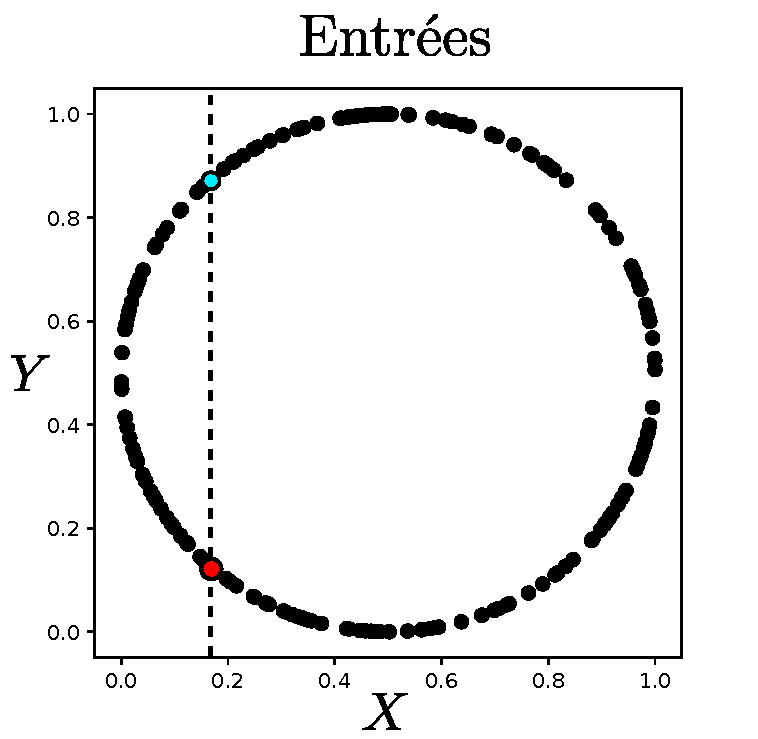
\includegraphics[width=0.8\textwidth]{2som_inp_noinformation}
    \end{minipage}
    \begin{minipage}{0.6\textwidth}
    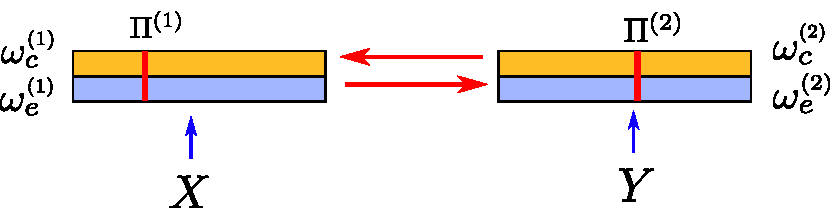
\includegraphics[width=\textwidth]{2som_archi}
    \end{minipage}
    \caption{\`A gauche, disposition des entrées dans l'exemple illustratif, sous forme de cercle. \`A droite, l'architecture de deux cartes en une dimension utilisée sur ces entrées afin d'illustrer les méthodes de représentation.\label{fig:exp}}
    \end{figure}

Les représentations que nous introduisons seront illustrées au long de ce chapitre sur l'exemple d'une architecture de deux cartes, comme présentée au chapitre~\ref{chap:modele}.
L'architecture est illustrée à droite en figure~\ref{fig:exp}~: elle est composée de deux cartes en une dimension. Chaque carte prend une entrée externe, correspondant à $\inpx\m{1}=x$ et $\inpx\m{2}=y$, l'abscisse et l'ordonnée de points 2D sur un cercle de centre $(x_c,y_c) = (0.5,0.5)$ et de rayon $0.5$.
Ces deux modalités sont dépendantes~: pour une même valeur de $x$, deux valeurs sont possibles pour $y$, et symétriquement. Ce modèle d'entrées est représenté sur le schéma de gauche, figure~\ref{fig:exp}.


Chaque carte est une ligne de 500 n\oe{}uds, indexés par une valeur $p\m{i} \in [0,1]$.
La carte $M\m{1}$ prend en entrée contextuelle la position du BMU $\bmu\m{2}$ de $M\m{2}$, et inversement~; chaque carte possède donc une couche de poids externes et une couche de poids contextuels. Les rayons de voisinage choisis sont $h_e = 0.2$ et $h_c = 0.02$.
Nous utiliserons également deux autres cartes de Kohonen 1D classiques en tant que témoin.
Ces cartes prennent les mêmes valeurs d'entrées $\inpx\m{1}$ et $\inpx\m{2}$ que les cartes de l'architecture CxSOM, mais ne sont pas connectées entre elles. 
Les paramètres de ces cartes indépendantes sont les mêmes que pour les cartes CxSOM~: chaque carte 1D compte 500 n\oe{}uds, le rayon de voisinage est constant $h_e = 0.2$. Ces cartes n'ont pas de couche de poids contextuels.
Cette expérience permet à la fois d'illustrer les représentations et de souligner les comportements qui diffèrent entre une carte classique et une carte placée au sein d'une architecture.



\subsection{Représentations et indicateurs classiques des cartes de Kohonen}
\begin{figure}[t]
    \begin{minipage}{0.5\textwidth}
    \centering
    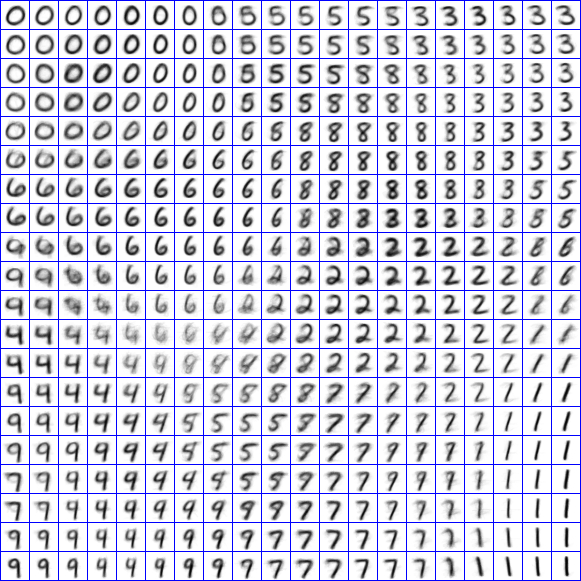
\includegraphics[width=0.65\textwidth]{digits.jpg}
    \end{minipage}
    \begin{minipage}{0.5\textwidth}
    \centering
    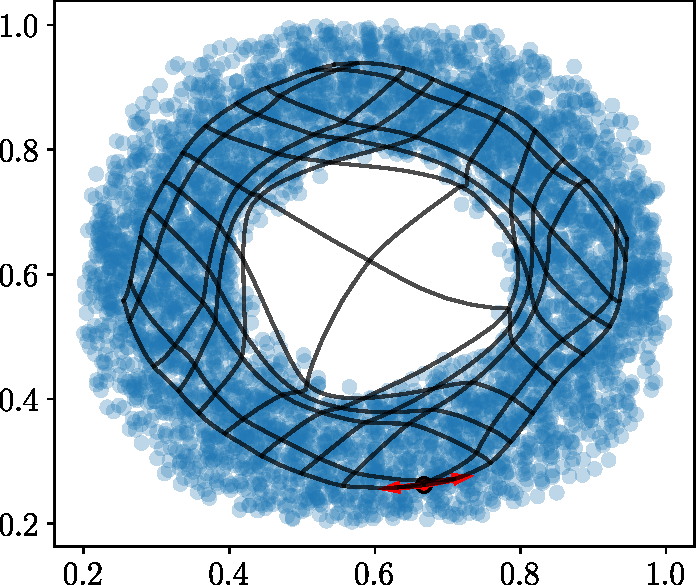
\includegraphics[width=0.7\textwidth]{points3.pdf}
    \end{minipage}
    \caption[Représentations classiques des poids d'une carte de Kohonen]{\label{fig:representation} Représentations possibles des poids d'une carte de Kohonen classique. \`A gauche, les prototypes qui sont des images $16\times 16$ sont tracées en fonction de leur position $p$ sur la grille~\footnotemark[1]. \`A droite, les prototypes sont des points en deux dimensions, qui sont tracés ainsi que la grille dans l'espace des entrées.}
    \end{figure}
    \footnotetext[1]{Source~: \href{https://frezza.pages.centralesupelec.fr/teachml2/Poly/Poly-ML-SDImetz.pdf}{polycopié d'apprentissage automatique} de CentraleSupélec Metz}


Les cartes de Kohonen sont particulièrement associées à une facilité de représentation et de visualisation. Leur nombre réduit de prototypes et leur topologie de faible dimension permet d'en tracer une représentation visuelle interprétable.

Deux représentations sont généralement privilégiées~:
\begin{itemize}
\item Les prototypes de chaque n\oe{}ud sont tracés à leur emplacement $p$ sur la carte. 
C'est le cas sur l'exemple de gauche en figure~\ref{fig:representation} dans lequel les poids des prototypes, qui sont des imagettes 16x16, sont affichés en chaque position de la carte en deux dimensions.
\item Lorsque les données apprises sont des points en deux ou trois dimensions, les poids des prototypes peuvent être directement tracés dans l'espace des entrées $\mathbb{R}^2$ ou $\mathbb{R}^3$. Les poids sont alors reliés en fonction des positions des n\oe{}uds dans la carte, montrant ainsi la déformation de la carte dans l'espace d'entrée. C'est le cas sur l'exemple de droite en figure~\ref{fig:representation} pour une grille en deux dimensions (en noir) ayant appris sur des entrées en deux dimensions (en bleu).
\end{itemize}



\subsection{Limites des représentations classiques dans le cas d'une architecture CxSOM}

Nous pouvons d'abord utiliser les représentations classiques mentionnées ci-dessus pour tracer les différentes couches de poids de chacune des cartes d'une architecture CxSOM à la fin de l'apprentissage.
La figure~\ref{fig:weights} présente le tracé des poids externes et contextuels des deux cartes de l'exemple selon leur position sur la carte, soit le pendant en une dimension de l'exemple de gauche en figure~\ref{fig:representation}.
La courbe orange correspond aux valeurs des poids externes de chaque carte.
Ce tracé permet d'observer que les poids externes couvrent l'intervalle $[0,1]$, et sont organisés de façon monotone, ce qui est l'organisation habituelle d'une carte classique se dépliant entre 0~et~1.
Les poids contextuels sont tracés en bleu. Ils ne présentent pas cette organisation monotone, mais font apparaître une organisation spatialement ordonnée~: deux prototypes proches ont des poids proches. Le tracé de poids nous informe donc sur leur caractère ordonné.

Toutefois, nous ne pouvons pas en tirer plus de conclusion.
La recherche de BMU dans CxSOM résulte d'un processus dynamique. La réponse de la carte n'est pas représentée par seulement ses poids, mais bien par ses BMU.
Par exemple, la représentation des poids de la figure~\ref{fig:weights} ne différencie pas les n\oe{}uds qui seront effectivement Best Matching Unit lors de l'apprentissage et des tests, des n\oe{}uds dits \emph{morts}.
Ces n\oe{}uds morts ont bien un poids, mais ne seront jamais BMU. Ils correspondent à des unités servant le processus d'organisation, mais pas l'encodage des entrées.

De plus, cette représentation concerne une seule carte. Nous ne pourrons pas tirer de conclusion sur l'influence des connexions entre cartes à partir de cette seule représentation.
Au regard des insuffisances des représentations classiques, déjà révélées sur un cas très simple de deux cartes mono-dimensionnelles, nous constatons qu'il est nécessaire de trouver un moyen de représenter l'architecture comme un tout. 
Nous devons ainsi définir des représentations supplémentaires qui montrent comment l'architecture de cartes est capable d'apprendre les relations entre les entrées multimodales.

\begin{figure}
\centering
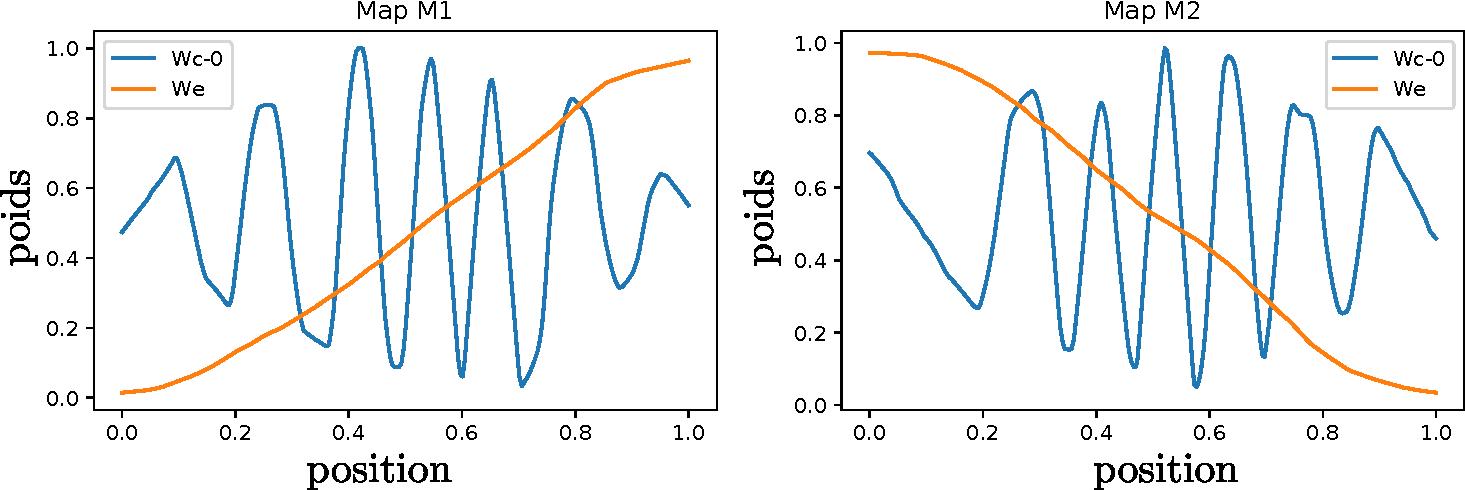
\includegraphics[width=0.9\textwidth]{weights_cercle1.pdf}
\caption{Représentation des valeurs des poids d'une carte au sein de CxSOM après apprentissage en fonction de leur position dans la carte. Les tracés des poids ne suffisent pas à donner une représentation de la réponse dynamique de la carte~; nous voulons pouvoir identifier les positions des Best Matching Units. \label{fig:weights}}
\end{figure}

Ce chapitre propose plusieurs façons de représenter une carte au sein d'une architecture.
Ces représentations seront illustrées sur l'exemple minimal de deux cartes.
Nous comparerons ici le comportement de l'architecture de deux cartes à celui de cartes classiques afin d'identifier des comportements d'apprentissage propres à CxSOM.
Nous utiliserons ensuite ces méthodes de représentation dans les chapitres suivants pour développer l'analyse du comportement d'apprentissage des cartes.

\section{Formalisation statistique des entrées et sorties des cartes}

En plus de s'intéresser à l'organisation des poids des cartes, nous utiliserons des représentations s'appuyant sur la réponse des cartes à des phases de test.
Pour formaliser ces réponses, nous choisissons de modéliser les entrées et les éléments des cartes de ces phases de test en tant que variables aléatoires.
Cette formalisation possède à la fois l'avantage de clarifier les représentations et de permettre le développement d'indicateurs statistiques sur l'apprentissage et l'encodage réalisé par les cartes.

\subsection{Formalisation des entrées}

Plaçons-nous dans le cas général d'une architecture de $n$ cartes.
Les entrées fournies à l'architecture sont $(\inpx\m{i} \in \mathcal{D}\m{i}, i = 1 \cdots D)$, tirées d'un ensemble d'espaces d'entrée $\mathcal{D}\m{1},\cdots,\mathcal{D}\m{D}$. 
Chaque espace $\mathcal{D}\m{i}$ est une \emph{modalité} de l'espace multimodal, avec $D$ le nombre de modalités considérées. Une carte peut ne pas prendre d'entrée externe, donc $D$ n'est pas forcément égal à $n$. 
Nous modélisons ces entrées $\inpx\m{i}$ comme des \emph{variables aléatoires} tirées selon une distribution $P\m{i}$ sur leur espace $\mathcal{D}\m{i}$.
$\mathbf{\inpx} = (\inpx\m{1}, \cdots, \inpx\m{D}) \in \mathcal{D}\m{1} \times \cdots \times \mathcal{D}\m{D}$ est la variable aléatoire jointe. 
Lors de chaque itération d'apprentissage, un vecteur $\mathbf{\inpx} = (\inpx\m{1}_t, \cdots , \inpx\m{D}_t)$ est présenté à l'architecture~: il s'agit d'une réalisation de la variable jointe $\mathbf{\inpx}$.

En pratique, ces variables sont des observations, issues par exemple de capteurs d'un robot. Ces observations sont issues d'un même environnement et sont liées par des relations au sein de cet d'environnement~: les variables $\inpx\m{i}$ ne sont généralement pas des variables indépendantes.
Le but de l'architecture est d'apprendre une représentation de ces entrées $\inpx\m{i}$ ainsi que de leurs dépendances.
Nous introduisons la notion de \emph{modèle d'entrées} pour référer à cette dépendance entre variables.
Dans l'exemple d'illustration, les modalités sont les abscisses $\inpx\m{1} = x$ et les ordonnées $\inpx\m{2} = y$~; le modèle d'entrées est le cercle sur lesquels sont situés les points, modélisé par exemple par l'équation $(x - 0.5)^2 + (y - 0.5)^2 = 0.5^2$.

\subsection{Formalisation du modèle d'entrées par une variable latente}\label{sec:U}

Afin de représenter les relations entre les entrées $\inpx\m{i}$ d'un modèle d'entrées, nous proposons d'introduire une nouvelle variable, que nous appelons $U$, et qui représente le modèle d'entrées dans sa globalité.
Sa valeur n'est pas fournie à l'architecture de cartes lors de l'apprentissage, il s'agit d'une variable latente.
Pour cela, nous définissons $U$ comme une variable paramétrant le modèle d'entrées et étant en bijection avec l'entrée jointe $(\inpx\m{1}, \cdots \inpx\m{n})$. 
De cette façon, $U$ conserve toute l'information sur le modèle d'entrées.
Une telle variable $U$ en bijection avec les entrées s'interprète par l'existence d'une variété de dimension inférieure ou égale à la dimension des entrées, sur laquelle sont positionnées les entrées multimodales.

Par exemple, les points de l'espace d'entrée pris en exemple, représentés à droite en figure~\ref{fig:U} sont positionnés sur une courbe 1D. Ils sont paramétrés par un angle.
Nous utilisons l'angle normalisé $U$ comme une variable 1D représentant ce modèle d'entrées~:
\begin{equation}
 \begin{cases}
     \inpx\m{1}= 0.5 + 0.5  \cos(2\pi U)\\
     \inpx\m{2} = 0.5 + 0.5 \sin(2 \pi U)
    \end{cases}\,
\end{equation}
En une seule valeur 1D, $U$ traduit la relation entre $\inpx\m{1}$ et $\inpx\m{2}$.

Nous pouvons étendre le cadre de choix de la variable latente en autorisant du bruit dans le modèle d'entrées.
Dans ce cas, 
\begin{equation}
    \forall i, \: \inpx\m{i} = f\m{i}(U) + \epsilon\m{i}
\end{equation}

L'utilisation de variables d'entrées multimodales placées sur une variété de dimension inférieure, est un cadre d'expériences généralisable. 
Il a en effet été proposé qu'en pratique, des variables en grande dimension, telles que des images, sont positionnées sur des variétés de dimension plus faible, dont un exemple tiré de~\cite{Pless2009ASO} est donné en figure~\ref{fig:U} 

Cette paramétrisation peut également être considérée comme un cas particulier de réduction de dimension des entrées sans perte d'information.
Les représentations proposées pourront également être adaptables à une variable $U$ obtenue par une méthode de réduction de dimension avec perte d'information (par exemple par une analyse en composantes principales).

\begin{figure}
    \begin{minipage}{0.4\textwidth}
    \centering
    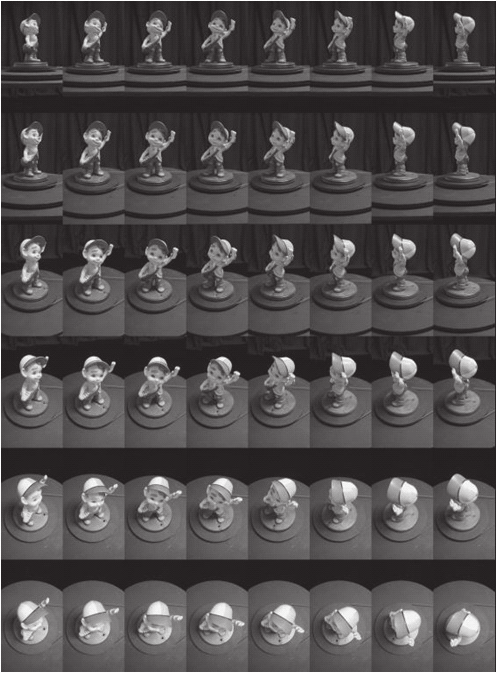
\includegraphics[width=0.8\textwidth]{pless-000.png}
    \end{minipage}
    \begin{minipage}{0.6\textwidth}
    \centering
    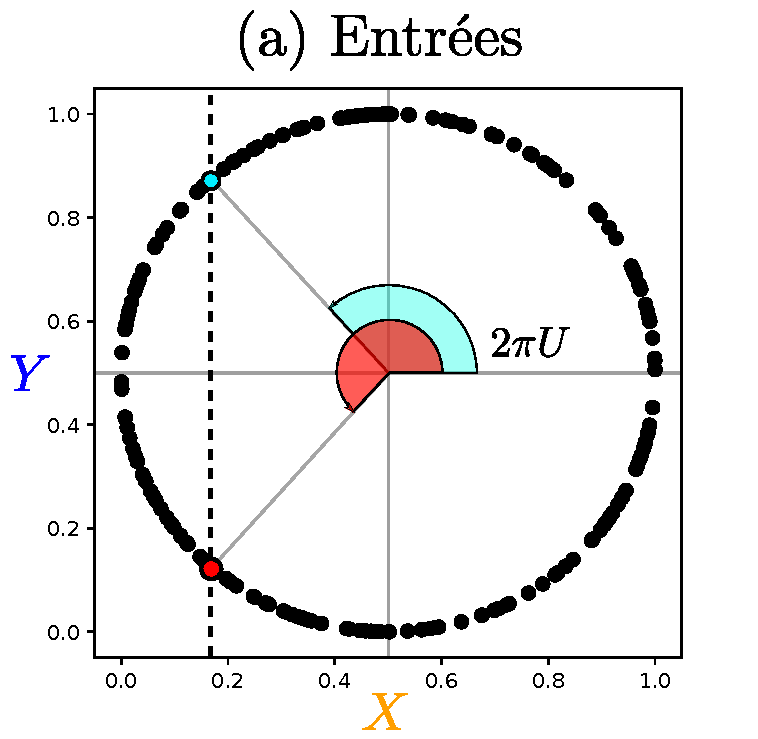
\includegraphics[width=0.9\textwidth]{2som_inp.pdf}
    \end{minipage}
    \caption{
        \`A gauche, ensemble d'images représentant une statuette sous différents angles de vue. Toutes les images, de grande dimension, sont situées sur une variété 3D sous-jacente représentant la rotation de la caméra. Source~:~\cite{Pless2009ASO}.
       La figure de droite présente le pendant en deux dimensions présentant également cette propriété. Les modalités 1D $\inpx\m{1}$ et $\inpx\m{2}$ sont placées sur un cercle qui est une variété en une dimension. Ce modèle est paramétré par la variable $U \in [0,1]$. Alors que les points rouge et bleu ont la même valeur pour $\inpx\m{1}$, ils sont bien différenciés par leur valeur de $U$.
       Nous utilisons ce modèle d'entrées comme exemple dans ce chapitre.
       \label{fig:U}}
\end{figure}

Nous cherchons, par l'architecture de cartes, à apprendre les entrées et les relations entre entrées~: nous cherchons donc à extraire une représentation du modèle d'entrées. La relation entre $U$ et $\mathbf{X}$ étant bijective, étudier comment l'architecture de cartes encode la variable latente $U$ équivaut à étudier comment l'architecture a appris le modèle d'entrées.

\subsection{Formalisation des éléments des cartes}

Afin d'étudier le comportement d'une carte à n'importe quel instant $t$ de l'apprentissage, nous effectuons des phases de test, décrites en figure~\ref{fig:flowchart} et déjà introduites en section \ref{sec:modele_test}. Lors d'une phase de test, les poids des cartes ne sont pas mis à jour. 
Les entrées utilisées lors du test sont un échantillon de la variable aléatoire $(\inpx\m{1}, \cdots, \inpx\m{n})$, de distribution identique à la distribution des entrées d'apprentissage.
La présentation d'une entrée engendre une recherche de BMU par relaxation et ainsi un ensemble d'éléments de réponse de la carte aux entrées. Ces éléments de réponse sont les activités externes et contextuelles, la position du BMU, les poids du BMU ou tout autre quantité observable à partir de l'état des cartes.

Nous avons représenté les entrées comme des variables aléatoires~; chaque élément de réponse des cartes d'une architecture à une phase de test peut également être considéré comme une variable aléatoire, car les poids ne sont pas mis à jour entre chaque itération de test.
Nous choisissons en particulier de nous intéresser aux positions des BMU $(\bmu\m{1}, \cdots, \bmu\m{n})$ et à leurs poids externes.
Toutes les valeurs obtenues lors d'une phase de test forment ainsi un échantillon de la variable aléatoire jointe suivante~:
$$(\underbrace{\inpx\m{1}, \cdots, \inpx\m{D}, U,}_{\text{Entrées}} \underbrace{\bmu\m{1}, \cdots, \bmu\m{n}, \w_e\m{1}(\bmu\m{1}), \cdots, \w_e\m{D}(\bmu\m{D})}_{\text{Eléments de réponse}})$$
Les composantes de cette variable jointe ne sont pas indépendantes. \'Etudier l'encodage des entrées par l'architecture de cartes consiste à étudier les dépendances se créant entre les composantes.
La représentation de la réponse des cartes s'effectue par le tracé des dépendances entre les composantes de la variable jointe définie ci-dessus.


Notons que les variables d'entrées sont à valeurs continues et $\bmu$ à valeurs discrètes, correspondant aux n\oe{}uds d'une carte.
Nous pourrons aussi considérer $\bmu$ comme une variable continue plutôt que discrète.
En effet, l'ensemble des positions d'une carte correspond à une discrétisation de l'espace continu $[0,1]$. Le déplacement par relaxation n'est par ailleurs pas limité aux positions discrètes des BMU.


Cette formalisation statistique des entrées et des réponses permettra aussi d'utiliser des outils et métriques issus de la théorie de l'information pour qualifier l'organisation des cartes au sein de l'architecture, ce que nous ferons dans le chapitre~\ref{chap:indicateur}.

\begin{figure}
\centering
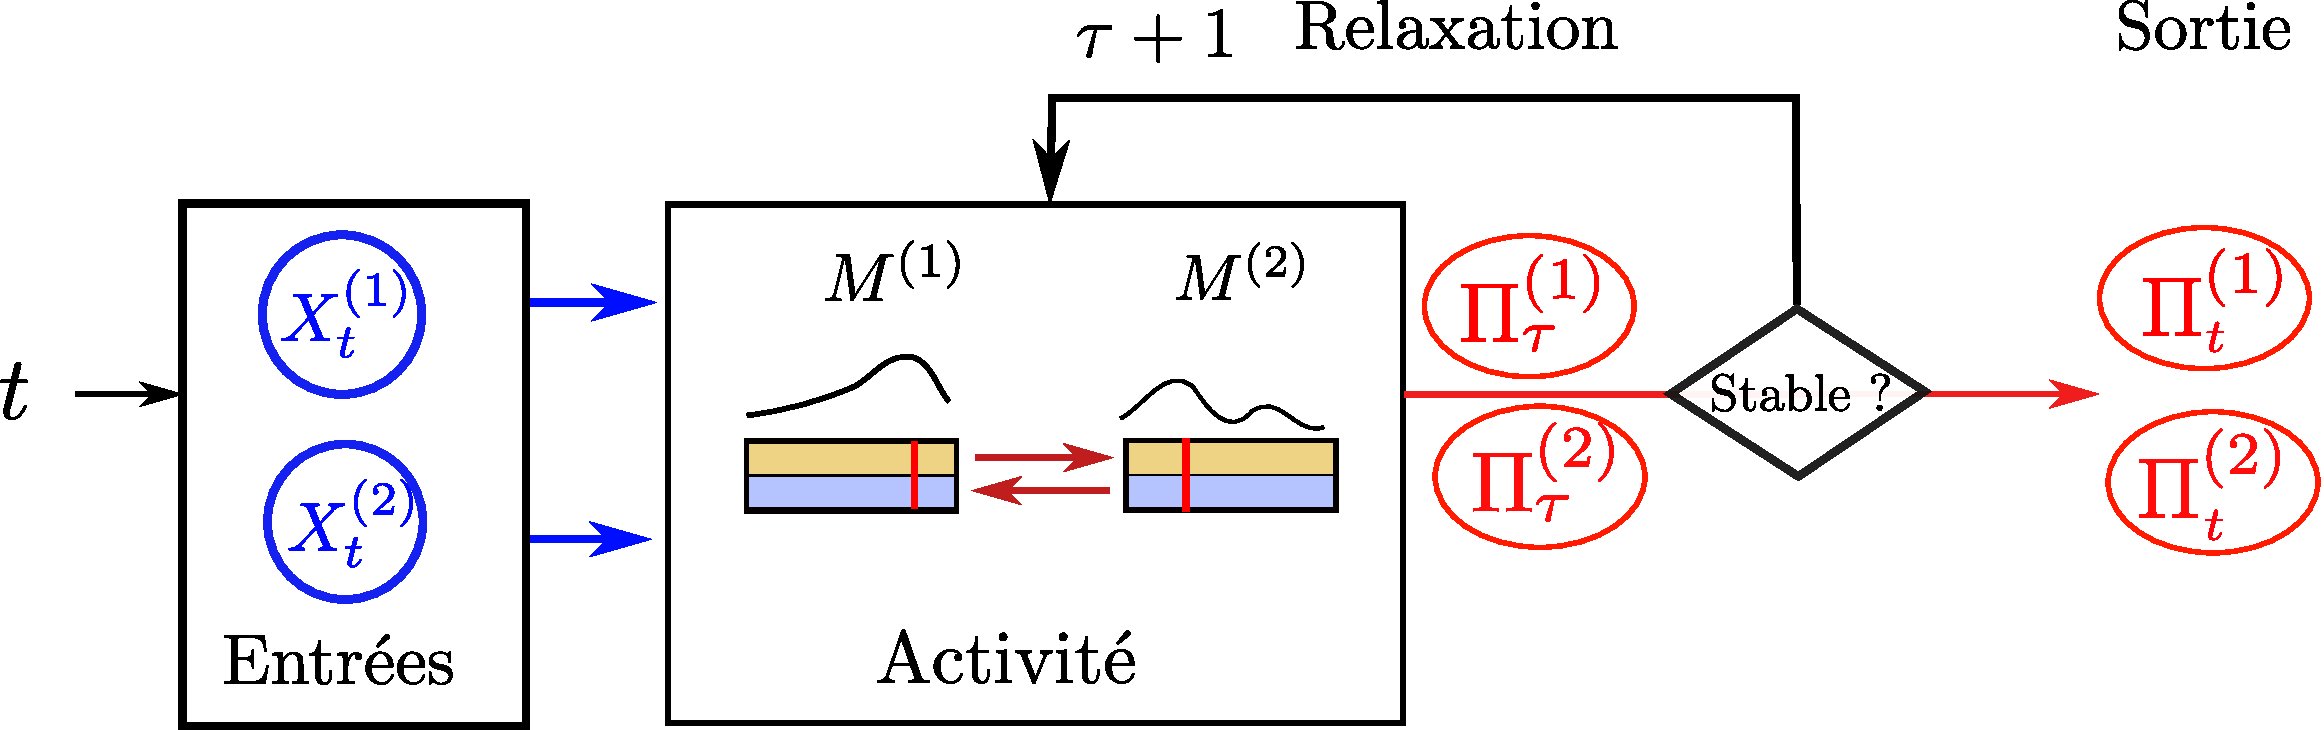
\includegraphics[width=0.85\textwidth]{tests_2maps.pdf}
\caption{Schéma décrivant une étape de test. Un test consiste à présenter successivement des réalisations de $\mathbf{X}$, notées $(\inpx\m{1}_t,\inpx\m{2}_t)$, et à effectuer la recherche de BMU par relaxation.
Contrairement à une phase d'apprentissage dans laquelle les poids sont mis à jour à partir des valeurs $\bmu_t$ obtenues après relaxation, ici nous considérons simplement les BMU $\bmu_t\m{1}$ et  $\bmu_t\m{2}$ comme sortie de l'architecture.
Les poids ne sont pas mis à jour entre chaque itération, ce qui permet de considérer une phase de test comme un échantillonnage de la variable aléatoire $(\inpx\m{1},\inpx\m{2}, U, \bmu\m{1}, \bmu\m{2}$).\label{fig:flowchart} }

\end{figure}

\section{Représentations graphiques}

Nous présentons dans cette section les représentations graphiques que nous utiliserons pour évaluer expérimentalement les architectures de cartes.
Ces représentations sont toutes un tracé des dépendances entre certaines composantes de la variable $$(\inpx\m{1}, \cdots, \inpx\m{D}, U, \bmu\m{1}, \cdots, \bmu\m{n}, \w_e\m{1}(\bmu\m{1}), \cdots, \w_e\m{D}(\bmu\m{D}))$$ dont un échantillon est obtenu lors d'un test.

\subsection{Erreur de quantification de l'entrée externe d'une carte}

La première fonction d'une carte de Kohonen est de réaliser une tâche de quantification vectorielle sur son entrée externe. 
Au sein d'une architecture de cartes, nous nous attendons à ce que chaque carte extraie une représentation de la modalité qu'elle prend comme entrée externe.
Afin d'étudier la qualité de quantification vectorielle au sein de chaque carte, nous traçons le nuage de points correspondant au poids externe du BMU $\w_e(\bmu\m{i})$ en fonction de l'entrée externe présentée $\inpx\m{i}$. 
Une carte effectue une quantification vectorielle correcte si ce nuage de points est proche de la fonction identité.
Ces tracés sont réalisés en figure~\ref{fig:erreur} pour l'expérience exemple. Ces tracés s'approchent de l'identité, ce qui montre que la quantification des entrées est correctement réalisée.
On pourrait également mesurer une erreur quadratique moyenne pour déterminer numériquement cette erreur de quantification, mais la représentation en nuage de points est, à défaut d'être quantitative, plus qualitative. 
En effet, ici, on observe que le nuage montre une structure \og en étages \fg{}. Nous reviendrons sur ce point par la suite, nous contentant de souligner ici que la représentation graphique exprime une propriété que la simple mesure d'erreur n'aurait pas mise en évidence.

Cette représentation nous informe sur la qualité de quantification dans une seule carte, relativement à une seule modalité. Cette seule représentation est insuffisante pour comprendre plus en détail le comportement d'une architecture de cartes~: il nous faut également définir des méthodes de représentation permettant d'évaluer comment la structure globale du modèle d'entrées est apprise par l'architecture dans son ensemble.

\begin{figure}
    \centering
    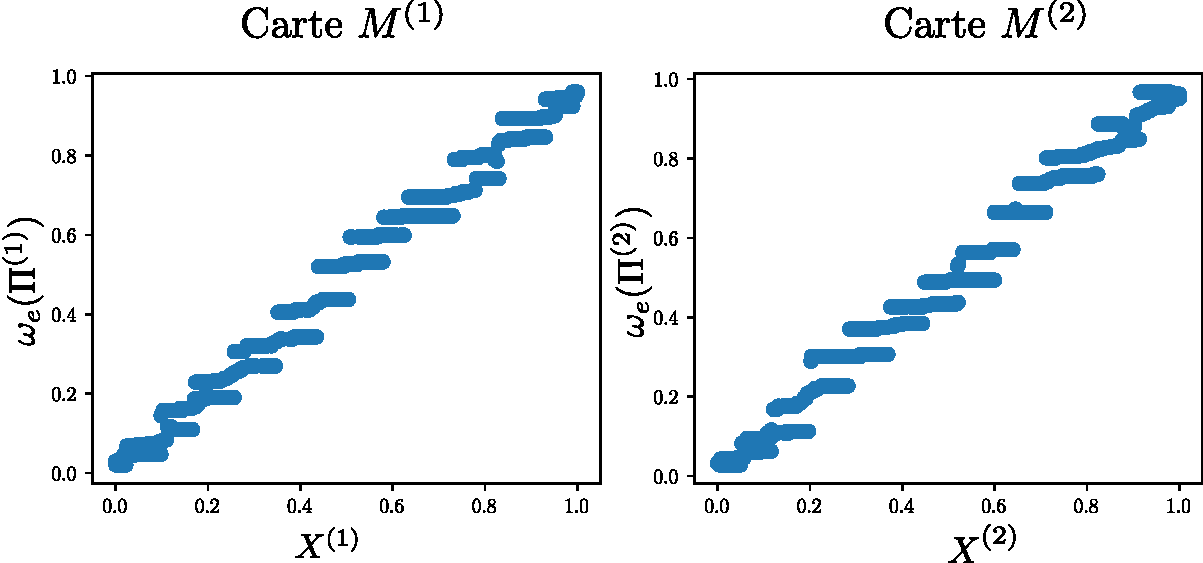
\includegraphics[width=0.7\textwidth]{w_x.pdf}
    \caption{Poids du BMU dans chaque carte en fonction de l'entrée présentée. On s'attend à des tracés proches de l'identité, indiquant que le poids du BMU d'une carte est une bonne représentation de l'entrée. 
    Ces tracés représentent une quantification vectorielle correctement réalisée, et font apparaître une structure en étages.
     \label{fig:erreur}}
\end{figure}

\subsection{Représentation cartographique des valeurs d'entrées préférentielles des BMU}

\begin{figure}
    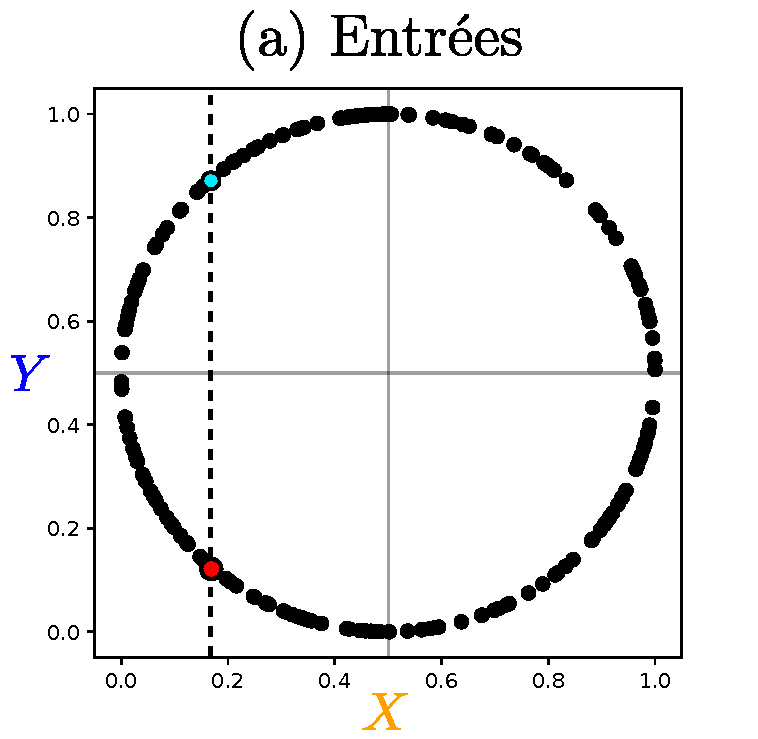
\includegraphics[width=\textwidth]{2som_inp_noU.pdf}
    \caption{Représentation cartographique des entrées $(\inpx\m{1},\inpx\m{2})$ d'une architecture de deux cartes, relativement au BMU de la carte $M\m{1}$ après apprentissage. 
    (a)~: entrées présentées à l'architecture. (b)~: poids et réponses d'une carte simple prenant $\inpx\m{1}$ en entrée. (c)~: poids et réponses de la carte $M\m{1}$ au sein de l'architecture de deux cartes.
    Nous constatons que les courbes de poids externes de chacune des cartes sont similaires. Les poids contextuels de CxSOM forment par contre des motifs pseudo-périodiques. La différence principale vient du choix du BMU~:
    les deux points bleu et rouge correspondent chacun à une valeur d'entrée. La réponse qui en résulte est reportée de la même couleur sur (b) et (c). Les deux points ont la même valeur pour $\inpx\m{1}$~: $x_1 = x_2 = 0.17$, mais leur valeur de $\inpx\m{2}$ est différente. 
    La carte simple représente ces deux entrées par une même position de BMU, tandis que la carte CxSOM distingue les BMU de ces deux points. \label{fig:inputs}}
    \end{figure}

Nous avons vu que la représentation des poids des cartes ne suffit pas à mettre en évidence la réponse de chaque carte. Nous proposons de tracer, pour chacune des cartes, les dépendances obtenues lors d'un échantillon de test entre toutes les entrées $(\inpx\m{1}, \cdots, \inpx\m{D})$ et le BMU $\bmu\m{i}$ de la carte. Le cas des cartes 1D et des entrées 1D permet de représenter toutes ces dépendances sur un même graphique.
Nous appelons ces tracés représentation cartographique des valeurs d'entrées.

En figure~\ref{fig:inputs}, nous avons tracé la représentation cartographique de $M\m{1}$ pour l'exemple à deux cartes, pour une carte au sein de CxSOM (c) et une carte simple prenant uniquement $\inpx\m{1}$ en entrée (b).
\begin{itemize}
    \item Les poids externes $w_e$ (en orange) et les poids contextuels $w_c$ (en bleu), sont tracés en fonction des positions $p$ dans la carte, ce qui correspond au tracé classique des poids représenté en figure~\ref{fig:weights}.
    \item Les entrées externes $\inpx\m{1}$ sont tracées en fonction de la position du BMU $\bmu\m{1}$, en bleu sur la figure.
    \item L'entrée externe $\inpx\m{2}$ est également tracée en fonction de $\bmu\m{1}$, en orange sur la figure. 
\end{itemize}

La représentation cartographique permet de visualiser directement la paire d'entrées $(\inpx\m{1}, \inpx\m{2})$ à laquelle un BMU $\bmu\m{1}$ a réagi.
Elle permet d'abord de constater que les points $(\bmu\m{1},\inpx\m{1})$ sont proches de la courbe des poids externes. Le poids externe du BMU est donc proche de l'entrée qui a été présentée et est une bonne approximation de cette entrée. 
Cela permet de conclure que la quantification vectorielle est bien réalisée dans cette carte sur les entrées externes, comme le montrait déjà la figure~\ref{fig:erreur}.

Ensuite, le tracé des échantillons de test permet d'observer la répartition des BMU sur une carte. 
L'organisation des poids externes de la carte $M\m{1}$ dans CxSOM (c) et de la carte $M\m{1}$ indépendante (b) est tout à fait semblable, différant seulement par le sens de variation de $\w_e$.
Grâce à l'ajout des positions de BMU, nous observons que dans CxSOM, la carte $M\m{1}$ est découpée en plusieurs zones dans lesquelles les unités sont BMU, séparées par des petites zones mortes, sans BMU. Ce phénomène n'est pas observé dans la carte classique, dans laquelle la plupart des positions de la carte sont BMU lors d'un test. 
Ce tracé permet ainsi d'identifier un comportement qui est spécifique à une architecture de cartes, par rapport à une carte classique. 

Enfin, les nuages de points orange et bleu, $(\bmu\m{1},\inpx\m{1})$ et $(\bmu\m{1},\inpx\m{2})$ permettent d'observer quelles valeurs d'entrées sont encodées à quelles positions dans chaque carte.
Par exemple, deux valeurs issues de l'échantillon de test sont mises en évidence en couleur rouge et bleu clair sur chaque graphique.
Ces deux points partagent la même valeur d'entrée $\inpx\m{1}$, mais leurs valeurs de $\inpx\m{2}$ sont différentes. Les réponses des cartes à ces deux entrées sont reportées de la même couleur sur les représentations cartographiques. Nous constatons que la carte simple répond par le même BMU à ces deux valeurs d'entrées. Dans CxSOM, la carte $M\m{1}$ répond avec des BMU différents, bien que les deux points aient la même valeur d'entrée externe. La représentation cartographique met en évidence ici que la réponse de la carte $M\m{1}$ s'effectue selon la valeur de $\inpx\m{1}$, mais également selon la valeur de $\inpx\m{2}$. 

Cette représentation permet ainsi de faire figurer les dépendances existant entre les BMUs et toutes les entrées, donc le modèle d'entrées, lors des phases de test. Elle met en avant l'organisation existant dans les réponses des cartes, non seulement dans l'organisation des poids.
Nous nous appuierons sur cette représentation dans les chapitres suivants pour généraliser les mécanismes d'organisation à plusieurs architectures et modèles d'entrées.

\subsection{Représentation de la variable latente selon les positions des BMU}\label{sec:u_bmu}

La représentation cartographique nous a permis de constater que sur chaque carte $M\m{i}$, les BMU se disposent selon les valeurs de l'entrée externe $\inpx\m{i}$, mais aussi selon les valeurs d'entrées des autres cartes, c'est-à-dire du modèle d'entrées.
Nous avons introduit en section~\ref{sec:U} une variable $U$ qui représente le modèle d'entrées. 
Nous proposons donc une autre manière de mettre en évidence le comportement d'organisation des BMU selon le modèle d'entrées, en réalisant le tracé de $U$ en fonction de la position du BMU correspondante $\bmu\m{i}$.

Cette représentation est réalisée en figure~\ref{fig:piu} pour l'exemple à deux cartes.
Ce tracé fait apparaître $U$ comme une fonction de la position du BMU dans chaque carte, contrairement au cas où les cartes ne sont pas connectées. 
L'existence de cette relation fonctionnelle traduit le fait que chaque carte a encodé le modèle d'entrées global et non seulement son entrée externe.

L'utilisation de $U$ permet ici de représenter, en une seule courbe, comment la carte a encodé les dépendances entre les entrées.
Cette représentation permet également de réduire la dimension des entrées à tracer et sera ainsi une représentation adaptée à des architectures de plus de cartes et des entrées de dimensions supérieures.

\begin{figure}
\centering
\includegraphics[width = \textwidth]{xu_yu_both.pdf}
\caption{Valeur de $U$ en fonction des valeurs du BMU $\bmu\m{i}$ dans chacune des cartes dans l'exemple d'illustration. Sur la première ligne, nous traçons la réponse de chaque carte dans le cas ou les deux cartes ne sont pas connectées. Sur la deuxième ligne, nous traçons la réponse de chaque carte après apprentissage du modèle d'entrées dans l'architecture.
Pour CxSOM, $U$ apparaît comme une fonction de la position du BMU $\bmu\m{i}$ dans chaque carte. Cette relation fonctionnelle est symbolisée par les pointillés sur les tracés du bas.
Les deux mêmes valeurs d'entrée tracées en figure~\ref{fig:inputs} sont également reportées sur ces tracés.
\label{fig:piu}}
\end{figure}

\subsection{Dépliement d'une carte dans l'espace d'entrée multimodal}

Une des représentations classiques des cartes de Kohonen est de tracer les poids de la carte dans l'espace de ses entrées, telle qu'en figure de droite en~\ref{fig:representation}. Cette représentation permet de faire apparaître un dépliement des poids d'une carte sur ses entrées.
De la même façon, nous voulons représenter comment chaque carte se déplie, non sur ses seules entrées externes, mais dans tout l'espace multimodal, ce qui est possible à partir des échantillons de test.

Nous proposons une façon de représenter le dépliement d'une seule carte de CxSOM dans l'espace global des entrées. Dans l'expérience illustrative, il s'agit donc de représenter comment une carte se déplie, mais dans l'espace 2D.
Au lieu de s'appuyer sur les poids des cartes, nous utilisons les poids externes des BMU obtenus lors du test. Cette représentation est tracée en ~\ref{fig:distortion} pour l'exemple à deux cartes.
Nous traçons sur cette figure le nuage de poids correspondant au poids des BMU selon leur position lors d'un test~: $ (\w_e\m{1}(\bmu\m{1}),\w_e\m{2}(\bmu\m{2}))$. 
Nous relions ces points selon l'ordre de leurs positions dans la carte $M\m{1}$ pour tracer $M\m{1}$, de même pour $M\m{2}$.  
Notons que les unités mortes ne peuvent pas être représentées sur la carte de cette façon. Nous ne représentons que les unités étant BMU. 

Comme les poids externes représentent directement la valeur de l'entrée externe, on s'attend à ce que la forme du nuage de points corresponde à la structure globale des entrées. Les valeurs représentées sont alors les valeurs quantifiées par l'architecture de cartes des entrées $(\inpx\m{1}, \inpx\m{2})$.
Ici, les tracés permettent de constater que le nombre de valeurs quantifiées est assez faible par rapport aux tailles des cartes~: on constate seulement 25 groupes de points quantifiant les points du cercle.
Par contre, le dépliement met en valeur la façon dont est parcouru l'espace dans chaque carte~: en fonction de $\inpx\m{1}$ dans la carte $M\m{1}$, et en fonction de $\inpx\m{2}$ dans la carte $M\m{2}$.

Cette représentation permet ainsi de visualiser comment l'espace d'entrée multimodal est quantifié, en fonction de la réponse de toutes les cartes.
Cette représentation offre également la possibilité de tracer comment une carte se déplie dans l'espace d'autres modalités que son entrée externe. 
Grâce à cette méthode, nous pouvons visualiser le dépliement d'une carte de l'architecture qui ne prendrait pas d'entrée externe.

\begin{figure}
    \begin{minipage}{0.49\textwidth}
    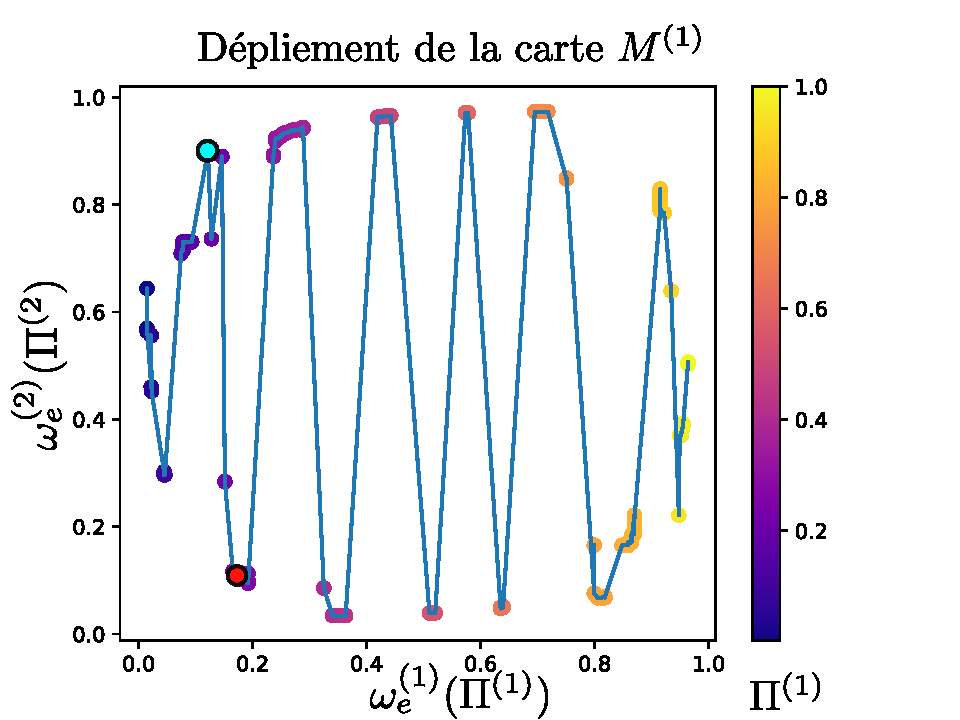
\includegraphics[width=\textwidth]{disto_cercle_M1.pdf}
    \end{minipage}
    \begin{minipage}{0.49\textwidth}
    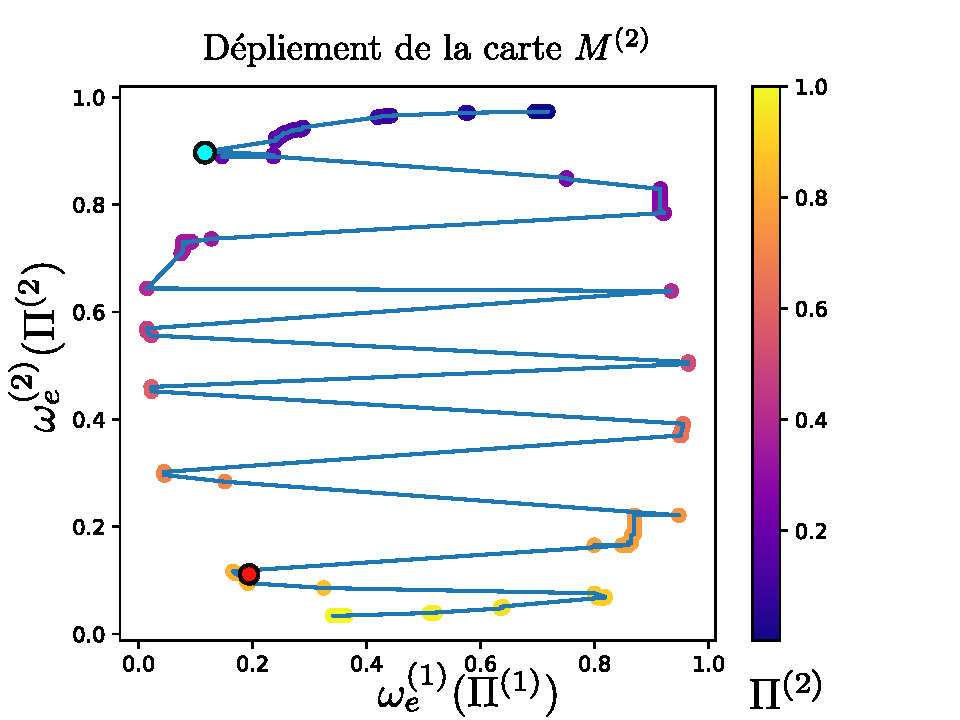
\includegraphics[width=\textwidth]{disto_cercle_M2.pdf}
    \end{minipage}
    \caption{Dépliement des cartes $M\m{1}$ et $M\m{2}$, reliés dans l'ordre de leurs positions selon $M\m{1}$ figure de gauche et $M\m{2}$ figure de droite. Le dépliement de chacune des cartes est alors représenté dans l'espace complet des entrées. L'indice du BMU est représenté par la carte de coloration, différenciant ainsi les deux extrémités des cartes correspondant aux positions 0 et 1.\label{fig:distortion}}
    \end{figure}

\section{Conclusion}

Dans ce chapitre, nous avons exposé la méthode d'analyse de l'architecture de cartes ainsi que les tracés que nous emploierons dans les expériences présentées par la suite. 
Nous avons souligné l'importance de faire apparaître une organisation dans les réponses des cartes en s'appuyant sur les BMU, plutôt que de représenter seulement leurs poids comme c'est généralement le cas dans l'étude des cartes auto-organisatrices classiques.

Nous avons d'abord proposé un cadre d'étude dans lequel les entrées et les réponses des cartes sont modélisées comme des variables aléatoires, échantillonnées durant des étapes de test qui peuvent être effectuées tout au long de l'apprentissage.
Nous avons également introduit une variable latente $U$ représentant le modèle d'entrées, qui permet de mettre en évidence les relations entre les entrées.


Les représentations que nous avons proposées sont ensuite simplement des tracés des dépendances entre les variables d'entrées et les réponses des cartes. Nous avons ainsi défini quatre représentations des cartes à partir d'un échantillon de test que nous utiliserons tout au long de cette thèse~:
\begin{itemize}
    \item Le tracé du poids du BMU en fonction de l'entrée externe permet d'évaluer la quantification vectorielle d'une carte (figure \ref{fig:erreur}).
    \item La représentation cartographique des entrées selon le BMU permet de faire apparaître quelles positions encodent quelles valeurs d'entrées. Elle permet de mettre en lien la disposition des poids et la réponse des cartes sur un même graphique. Elle sert à visualiser l'organisation des réponses des cartes, grâce aux positions des BMU (figure~\ref{fig:inputs}).
    \item Le tracé de la variable $U$ selon les positions des BMU d'une carte $\bmu\m{i}$ résume la représentation cartographique des entrées et fait directement apparaître comment le modèle d'entrées est encodé par la position du BMU.
    Nous observons en particulier que l'apprentissage du modèle d'entrées se traduit par l'observation d'une relation fonctionnelle entre $U$ et $\bmu\m{i}$ dans chaque carte (figure \ref{fig:piu}).
    \item Enfin, nous avons présenté une représentation du dépliement de chaque carte dans l'espace de toutes les entrées en traçant les poids externes des BMU de l'architecture, ordonnés selon les valeurs des positions dans une des cartes. Cette représentation apporte une vision de la réponse générale de l'architecture et non seulement d'une carte. Elle permet également de représenter les réponses des cartes ne prenant pas d'entrée externe. (figure \ref{fig:distortion}).
\end{itemize}

Ces tracés, réalisés sur un exemple d'expérience à deux cartes, ont mis en évidence une différence notable entre la réponse d'une carte au sein d'une architecture CxSOM et une carte classique~: dans CxSOM, chaque carte définit son BMU non seulement en fonction de son entrée externe, mais également selon l'entrée qui a été présentée à l'autre carte. Ce comportement était attendu, car le BMU est choisi en fonction de l'entrée externe et de l'entrée contextuelle d'une carte. Les tracés permettent par contre de constater une organisation particulière et étonnante dans les réponses des cartes~: une carte se divise en zones de BMU, séparées par des zones mortes.

L'analyse plus approfondie de ces mécanismes d'organisation dans les réponses des cartes est l'objet du chapitre~\ref{chap:analyse}. Nous nous appuierons pour cela sur les représentations que nous venons de présenter.
Ensuite, même avec des représentations adaptées, l'analyse d'architectures comportant de nombreuses cartes ne peut pas simplement s'effectuer à l'aide de représentations graphiques, qui deviendraient trop chargées. 
Cette difficulté de représentation et le besoin de comparer des expériences entre elles soulève la nécessité de définir des indicateurs numériques du fonctionnement d'une carte, que nous proposerons au chapitre~\ref{chap:indicateur} à partir de la formalisation des entrées et réponses des cartes sous forme de variables aléatoires.

\ifSubfilesClassLoaded{
    \printbibliography
    %\externaldocument{../main.tex}   
}{}
\end{document}

% En biologie, les aires du cortex cérébral sont cartographiées en faisant varier le motif d'entrée dans son espace, et en indiquant pour chaque position sur la surface corticale, la valeur d'entrée préférentielle à laquelle elle réagit. Cela donne alors une représentation cartographique où des valeurs de l'espace d'entrée sont tracées par rapport à la position sur le substrat neuronal du neurone qui y réagit.
% Par exemple, une carte corticale est tracée pour l'aire visuelle primaire du cortex cérébrale, l'aire v1, en figure~\ref{fig:v1_repr}.

% \begin{figure}
%     \centering
%     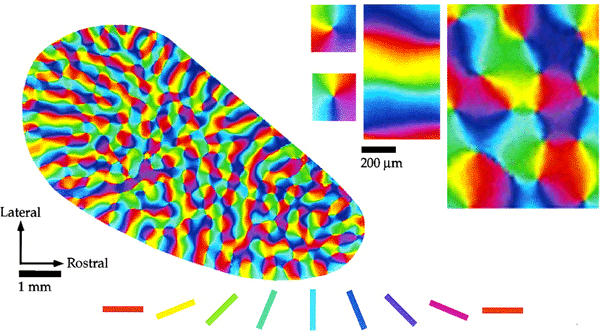
\includegraphics[width=0.7\textwidth]{v1.jpg}
%     \caption{Carte corticale de l'aire cérébrale visuelle V1. Pour tracer cette représentation, un ensemble de traits de différentes orientations sont présentés en stimuli visuels au sujet, indiqués en bas de l'image. Le neurone réagissant à une entrée d'orientation particulière est coloré sur la carte de la couleur correspondante à l'entrée. Cette méthode permet de tracer des cartes corticales d'une aire cérébrale \cite{Bosking1997OrientationSA}. \label{fig:v1_repr}}
% \end{figure}
